We use the KUKA youBot omni-directional mobile platform, which is equipped with a 5 DOF manipulator (Figure~\ref{fig:youBot}). At the end effector of the manipulator an Intel RealSense camera with a motion sensor has been mounted. Next to the camera we replaced the standard gripper from youBot with an also youBots soft two-finger gripper. 
Thanks to it we are able to grasp bigger and more complex objects more precisely.

A Hokuyo URG-04LX-UG01 laser scanner at the front of the youBot platform is used for localization and navigation. 
We are planning to add a second laser scanner of the same type on the back of the robot. This improves localization quality and ensures better obstacle avoidance, mainly when driving backwards with the robot.

\newpage
Last year we used the internal computer, together with an external ASUS Mini PC (4 GB RAM, Intel Core i3). We used the internal computer in the youBot to start-up the motors and also for the SLAM. This was a huge error because we added an enormous data transfer between the two computers, what slowed down the complete system. 
To avoid the communication problems and latency between them both, we decided to run everything, except the motor drivers, on the external PC. We also replace the slow i3 for a more powerful CPU Intel Core i7-4790K, 4x 4.00 GHz. Table~\ref{tab:hw} shows our new hardware specifications.

For connecting the two PCs we use a router mounted on the back of youBot. With external machines we can connect to the routers network and communicate with both PCs on the youBot.

We also added an Inertial Measurement Unit~(IMU) to gather information about the heading of the platform. On the IMU runs a fusion algorithm which provides the orientation of the platform as quaternion or Euler angles.

\begin{figure}[htbp]
	\begin{minipage}{0.45\textwidth}
		%\vspace{2.4cm}
		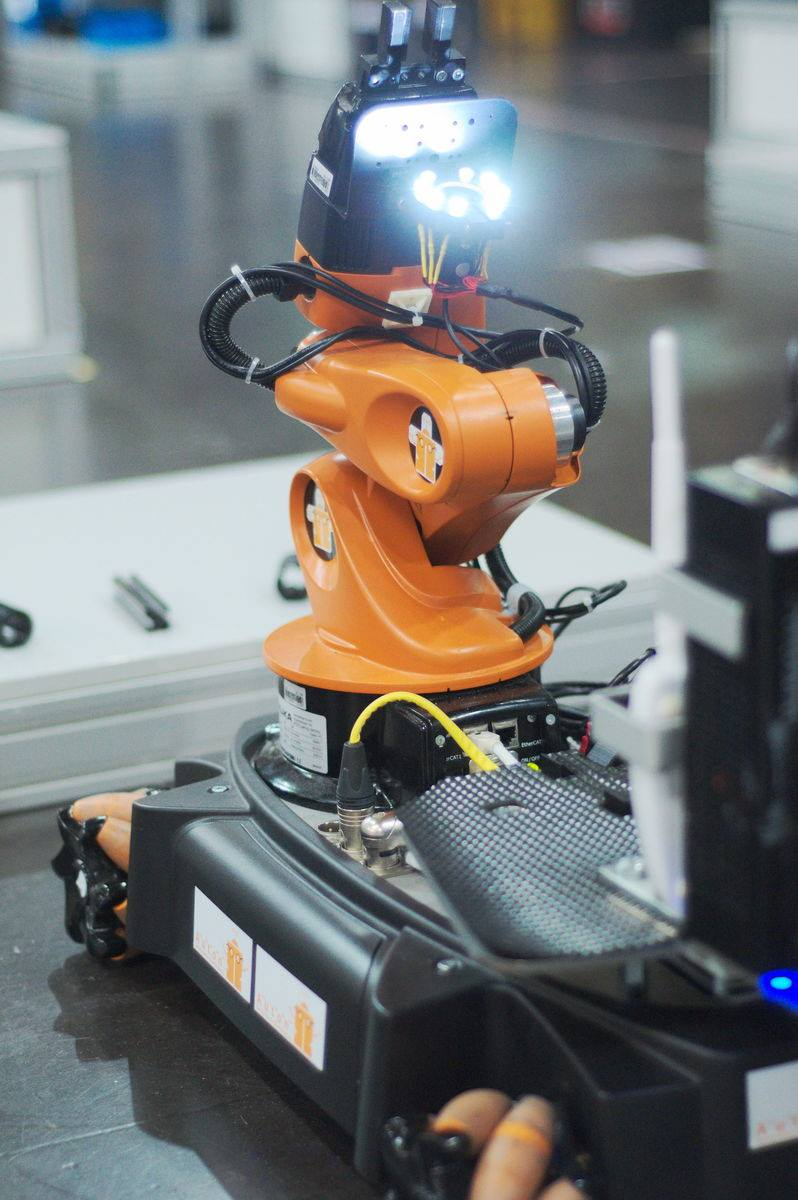
\includegraphics[width=\textwidth]{img/YoubotInAction.jpg}
		\caption{KUKA youBot Plattform}
		\label{fig:youBot}
	\end{minipage}
	\hfill
	\begin{minipage}{0.45\textwidth}
		\renewcommand*\figurename{Tab.}
		\setcounter{figure}{0}
		%	\begin{table}[htbp]
		\centering
		\caption{Hardware Specifications}
		\begin{tabular}{ | p{2cm} | p{3cm} | }
			\hline
			\bfseries{PC 1} &  \\
			\hline
			CPU & Intel i7-4790 \\
			RAM & 16 GB DDR3 \\
			Storage & SSD 128 GB \\
			OS & Ubuntu 14.04 \\
			\hline \hline
			\bfseries{PC 2} &  \\
			\hline
			CPU & Intel Atom D510 \\
			RAM & 2 GB DDR2 \\
			Storage & SSD 32 GB \\
			OS & Lubuntu 14.04 \\
			\hline \hline
			\bfseries{Grasp} &  \\
			\hline
			Type & soft, two-finger \\
			Stroke & 20 mm \\
			\hline \hline
			\bfseries{Lidar} &  \\
			\hline
			Type & Hokuyo URG-04LX \\
			Range & 5.6 m \\
			Resolution & 0.352 deg \\
			\hline \hline
			\bfseries{Router} &  \\
			\hline
			Type & Edimax 2.4/5 GHz \\
			\hline \hline
			\bfseries{IMU} &  \\
			\hline
			Type & BNO055 Bosch \\
			DOF & 9 \\
			Rate & 30 Hz (ROS) \\
			\hline
		\end{tabular}
		\label{tab:hw}
	\end{minipage}
\end{figure}

\setcounter{figure}{1}

